%% Manuscript for the effect of designed conversational architecture on the perception of agents
%%
%% The first command in your LaTeX source must be the \documentclass command.
\documentclass[sigconf,screen,review, anonymous]{acmart}

\usepackage[linewidth=1pt]{mdframed}
\usepackage{lipsum}

\newcommand{\cmt}[1]{}%{\ignorespaces}


%% NOTE that a single column version may be required for 
%% submission and peer review. This can be done by changing
%% the \doucmentclass[...]{acmart} in this template to 
%% \documentclass[manuscript,screen]{acmart}
%% 
%% To ensure 100% compatibility, please check the white list of
%% approved LaTeX packages to be used with the Master Article Template at
%% https://www.acm.org/publications/taps/whitelist-of-latex-packages 
%% before creating your document. The white list page provides 
%% information on how to submit additional LaTeX packages for 
%% review and adoption.
%% Fonts used in the template cannot be substituted; margin 
%% adjustments are not allowed.
%%
%%
%% \BibTeX command to typeset BibTeX logo in the docs
\AtBeginDocument{%
  \providecommand\BibTeX{{%
    \normalfont B\kern-0.5em{\scshape i\kern-0.25em b}\kern-0.8em\TeX}}}

%% Rights management information.  This information is sent to you
%% when you complete the rights form.  These commands have SAMPLE
%% values in them; it is your responsibility as an author to replace
%% the commands and values with those provided to you when you
%% complete the rights form.
\setcopyright{acmcopyright}
\copyrightyear{2023}
\acmYear{2023}
\acmDOI{XXXXXXX.XXXXXXX}

%% These commands are for a PROCEEDINGS abstract or paper.
\acmConference[Conference acronym 'XX]{Make sure to enter the correct
  conference title from your rights confirmation email}{June 03--05,
  2018}{Woodstock, NY}
%
%  Uncomment \acmBooktitle if th title of the proceedings is different
%  from ``Proceedings of ...''!
%
%\acmBooktitle{Woodstock '18: ACM Symposium on Neural Gaze Detection,
%  June 03--05, 2018, Woodstock, NY} 
\acmPrice{15.00}
\acmISBN{978-1-4503-XXXX-X/18/06}

%%
%% Submission ID.
%% Use this when submitting an article to a sponsored event. You'll
%% receive a unique submission ID from the organizers
%% of the event, and this ID should be used as the parameter to this command.
%%\acmSubmissionID{123-A56-BU3}

%%
%% end of the preamble, start of the body of the document source.
\begin{document}
%TC:ignore

%%
%% The "title" command has an optional parameter,
%% allowing the author to define a "short title" to be used in page headers.
% \title[short title]{How to Make Pinocchio a Real Boy? Designing conversational architecture elements to achieve desirable anthropomorphized perceptions}
\title[Bot's Guide to Being Human]{Bot's Guide to Being Human: Investigating the Effect of Conversational Architecture Elements on the Anthropomorphized Perceptions of Conversational Agents}
% Blurring the line between human and bots


%%
%% The "author" command and its associated commands are used to define
%% the authors and their affiliations.
%% Of note is the shared affiliation of the first two authors, and the
%% "authornote" and "authornotemark" commands
%% used to denote shared contribution to the research.
\author{Christina Wei}
\email{christina.wei@mail.utoronto.ca}
\affiliation{%
  \institution{University of Toronto}
  \city{Toronto}
  \country{Canada}
}

\author{Young-Ho Kim}
\email{ygho.kim@navercorp.com}
\affiliation{%
  \institution{Naver Corporation}
  \city{Seoul}
  \country{Korea}
}

\author{Anastasia Kuzminykh}
\email{anastasia.kuzminykh@utoronto.ca}
\affiliation{%
  \institution{University of Toronto}
  \city{Toronto}
  \country{Canada}
}

%%
%% By default, the full list of authors will be used in the page
%% headers. Often, this list is too long, and will overlap
%% other information printed in the page headers. This command allows
%% the author to define a more concise list
%% of authors' names for this purpose.
\renewcommand{\shortauthors}{Wei, Kim, and Kuzminykh}

%%
%% The abstract is a short summary of the work to be presented in the
%% article.
\begin{abstract}
  TBD
\end{abstract}

%%
%% The code below is generated by the tool at http://dl.acm.org/ccs.cfm.
%% Please copy and paste the code instead of the example below.
%%
\begin{CCSXML}
<ccs2012>
 <concept>
  <concept_id>10010520.10010553.10010562</concept_id>
  <concept_desc>Computer systems organization~Embedded systems</concept_desc>
  <concept_significance>500</concept_significance>
 </concept>
 <concept>
  <concept_id>10010520.10010575.10010755</concept_id>
  <concept_desc>Computer systems organization~Redundancy</concept_desc>
  <concept_significance>300</concept_significance>
 </concept>
 <concept>
  <concept_id>10010520.10010553.10010554</concept_id>
  <concept_desc>Computer systems organization~Robotics</concept_desc>
  <concept_significance>100</concept_significance>
 </concept>
 <concept>
  <concept_id>10003033.10003083.10003095</concept_id>
  <concept_desc>Networks~Network reliability</concept_desc>
  <concept_significance>100</concept_significance>
 </concept>
</ccs2012>
\end{CCSXML}

\ccsdesc[500]{Computer systems organization~Embedded systems}
\ccsdesc[300]{Computer systems organization~Redundancy}
\ccsdesc{Computer systems organization~Robotics}
\ccsdesc[100]{Networks~Network reliability}

%%
%% Keywords. The author(s) should pick words that accurately describe
%% the work being presented. Separate the keywords with commas.
\keywords{conversational agents, user perception, conversational architecture, social cues}

%%\received{20 February 2007}
%%\received[revised]{12 March 2009}
%%\received[accepted]{5 June 2009}

%%
%% This command processes the author and affiliation and title
%% information and builds the first part of the formatted document.
\maketitle
%TC:endignore

\section{Introduction}

Conversational agents (CAs) are software-based systems, either voice of text-based, designed to interact with humans using natural language. Adoption for CAs such as Alexa (Amazon) or Siri (Apple) are rapidly growing in the market, with half of US internet users own one or more smart speaker devices \cite{2022comscore}. These conversational agents are designed to be ubiquitous, easily accessible through smartphones, tablets, laptops and smart devices. Because these agents leverage natural language for interaction, they solicit social responses from users, encouraging users to attribute lifelike qualities, a.k.a. anthropomorphized perceptions to CAs \cite{eyssel2012if}.

Anthropomorphism is defined as the attribution of traits that we typically associate with being distinctly human to nonhuman entities \cite{waytz2010sees}. For example, users tend to personify conversational agents like Amazon Alexa by using person pronouns instead of object pronouns in online reviews \cite{purington2017alexa}.  Research shows that anthropomorphic design is beneficial to establishing and maintaining trust between users and conversational agents \cite{seeger2021chatbots}. Also, speakers tend to align their lexical choices with conversational agents, similar to human-human conversations \cite{cowan2015does}. Anthropomorphism has been shown to ease user interactions, e.g. making agents more approachable, engaging, and trustworthy when they exhibit human characteristics \cite{qiu2009evaluating}. These processes are of particular interest for human-agent communication because they form the basis for user expectations and predispositions regarding agents' behavior, reliability of the information, etc. \cite{kuzminykh2020genie}.

One of the key factors for anthropomorphized perception is how conversational agents convey information through verbal or non-verbal cues. Studies have found that conversational agents are perceived as more socially present and emotionally intelligent if they use sentiment-adaptive response based on user's utterances, resulting in higher user satisfaction \cite{diederich2019emulating} \cite{yang2017perceived}. Also, CAs that mimic user behaviour through lexical alignment reduce users' cognitive workload, resulting in higher engagement with the interaction \cite{spillner2021talk}. Non-verbal cues such as expressive prosody contribute to higher perceived intimacy with the user, as well as higher perceived enjoyment and ease of use \cite{kim2020can}. However, conversational architecture design may lead to negative consequences, such as an agent with an extroverted personality may be seen as less trustworthy, as users are irritated by the system's overly familiar attitude \cite{andrews2012system}.

Even though there are existing research efforts investigating the effect of various conversational architecture elements on the anthropomorphized perception of agents, there is no clear view on the overall landscape on the state of research to understand what has been studied and what needs more efforts. Some reasons for this gap could be due to the lack of consistency in perception measures such as humanness or empathy. There are various questionnaires used in the studies (e.g. Godspeed Questionnaire) but their definitions for perceptions may be different. Also, there are various confounding factors like prior experience and domain of usage that makes it hard to generalize design principles for anthropomorphized perception of agents.

This paper attempts to address this gap in knowledge by investigating the following research questions: (RQ1) How does the specifics of conversational architecture design affect the anthropomorphized perception of CAs? and (RQ2) How does the specifics of conversational architecture design affect the perception of interaction with CAs? Through a comprehensive review of the existing literature, this paper presents the synthesis of a design framework developed based on X number of paper published between 2010 and 2022. The framework associated four categories of perception - interaction, ability of the agent, human attributes of the agent, and social connections with the user, with four categories of conversational architecture elements - verbal (content, style), visual (CMC), auditory (voice qualities, vocalizations), and chronemics adapted from Feine et al \cite{feine2019taxonomy}.

<One paragraph summarizing results>

<One paragraph outlining contributions to the HCI community>
* Synthesize existing framework into design framework \newline
* Point out gaps in research \newline

In the remainder of the paper, we first review the existing literature on design frameworks for conversational agents and measures of anthropomorphized perceptions. We then describe our literature review and data analysis process, following by describing the design framework synthesized based on findings of the collected literature corpus. Finally, we discuss the critical gaps in research identified through our analysis, and propose key opportunities for future research.

\section{Literature Review}

Synthesis on conversational architecture

Synthesis on measures

Connections between conversational architecture elements and measures


\section{Methods}

\subsection{Search Procedure}

We reviewed and selected relevant literature related to designed conversational architecture elements and perceptions of conversational agent following PRISMA guidelines \cite{prisma}. Searches were carried out in the ACM Digital Library between January 1 and January 15, 2023. Based on search terms used in previously published literature reviews on conversational agents \cite{clark2019state}\cite{rapp2021human} , the following keywords have been identified to search for publications related to conversational user interfaces:
\newline

\begin{mdframed}
"conversational agent" OR "natural language interface" OR "IPA" OR "intelligent personal assistant" OR "chatbot" OR "speech interface" OR "voice assistant" OR "intelligent agent" OR "human-chatbot communication" OR "virtual agent" OR "dialog* system" OR "voice user interface" OR "human computer dialog*"
\end{mdframed}

\subsection{Selection Criteria}
The initial query retrieved 2901 unique publications. The following selection criteria are applied to identify literature related to the effect of conversational architecture on perception of agents:
\begin{itemize}
  \item Peer-reviewed publications written in English
  \item Voice-based or text-based disembodied conversational agents
  \item Interaction study on the impact of designed conversational architecture elements on the perception of agents.
  \item Users must interact with conversational agent in the study. Observer studies are excluded from the corpus
  \item Measures the perceptions of the interaction or perceptions of the agent as part of the study
\end{itemize}

We screened the titles and abstracts of the papers based on the selection criteria below which resulted in 221 papers. Reviewing the full articles of these publication resulted in <X> papers for analysis. A backward/forward search was also performed to find new publications, adding <X> papers to the corpus.

<Add graphic of PRIMSA process>

\subsection{Data Analysis}

Categorization of perceptions \newline
Categorization of social cues \newline

\subsection{Dataset Characteristics}
* Year and publication venue
\newline
* Modality - voice vs. text
\newline
* Systems tested - WoZ, prototype, actual applications

\section{Framework}
%Wrote based on papers up to [60], 25 papers

\begin{figure*}[h]
  \centering
  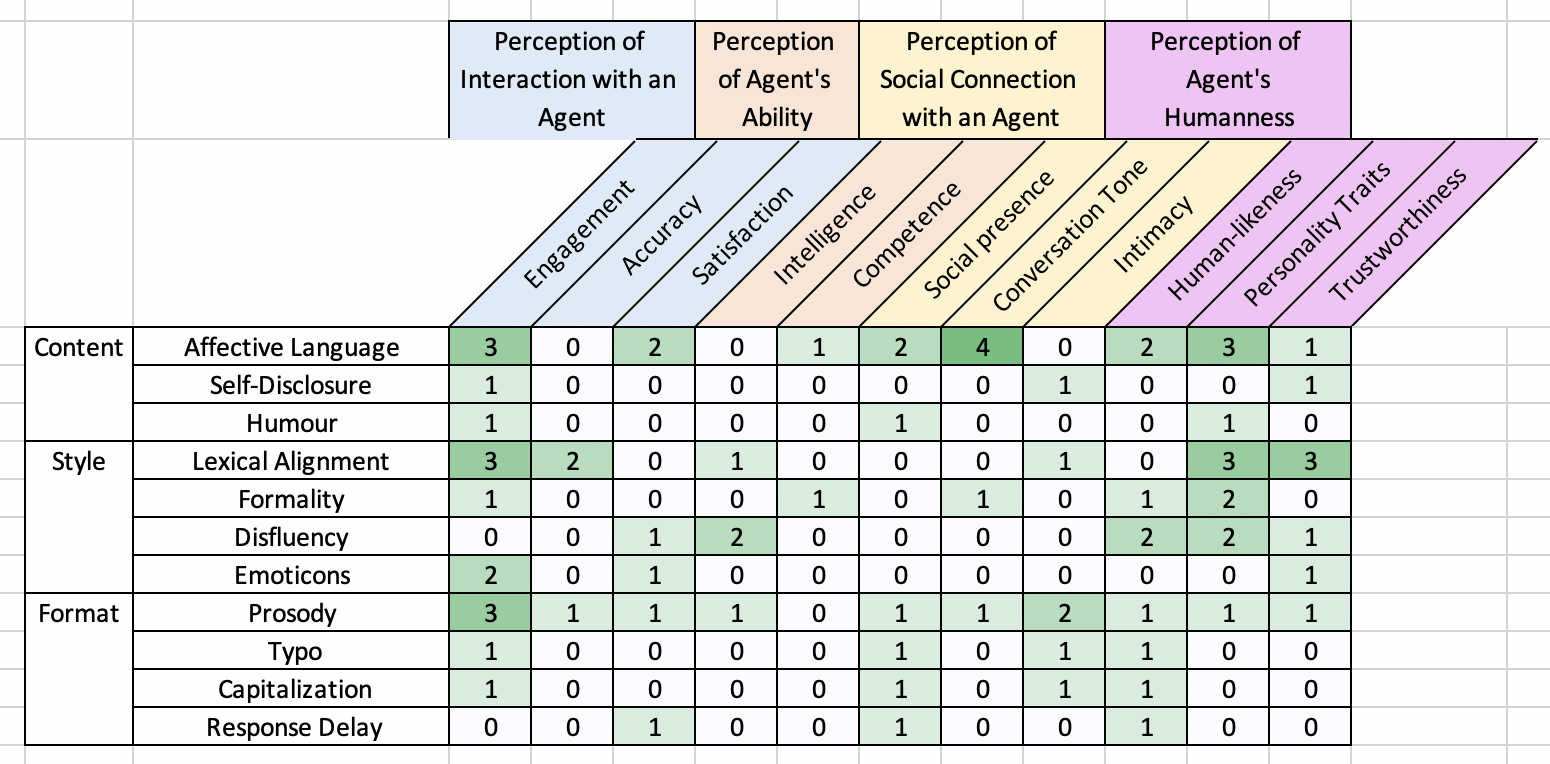
\includegraphics[width=\textwidth]{heatmap.png}
  \caption{Heatmap of literature for perception of conversational agents for each type of conversational architecture element.}
  \Description{This graph shows the number of papers measuring the effect of conversational architecture elements on different perception measures of conversational agents. Conversational architecture elements are categorized into content (affective language, self-disclosure, humour), format (disfluency, typo, capitalization, speech rate, response delay), and style (lexical alignment, formality, emoticons, prosody). Perceptions are categorized into perception of interaction with an agent (engagement, satisfaction, accuracy), perception of social connection with an agent (intimacy, conversation tone, social presence), and perception of agent's humanness (human-likeness, trustworthiness, personality traits).}
  \label{fig:heatmap}
\end{figure*}

Figure \ref{fig:heatmap}


%%%%%
\subsection{Perception of Interaction with an Agent}
%%%%%

This section discusses user's perception of their interaction with a conversational agent. Engagement, accuracy, and satisfaction are the three variables used to evaluate how people perceive interactions with CAs. \textit{Engagement} measures user's attitude towards the task they are achieving through working with the agent, including how easy it is to use the system and its perceived usefulness, convenience and helpfulness for the user. Additionally, it includes the user's emotional responses to the interaction, such as annoyance, enjoyment, and irritation. \textit{Accuracy} measures whether the agent was perceived to be able to provide the correct answers in response to the user. \textit{Satisfaction} measures the whether the agent was able to fulfill user's expectations through the interaction encounter.

Out of the list of publications that were evaluated, there is a good coverage on the effect of conversational architecture elements on the perception of interaction with an agent. Out of the three factors, engagement is the most frequently used measure to assess interaction quality, followed by satisfaction. Perceived accuracy of the agent is rarely used within literature, with only a few papers measuring this perception. 

[TODO] * Associations between conversational architecture elements and perceptions
For both text and voice modalities, lexical alignment had a positive effect on engagement by decreasing the cognitive load of users. 

%%
\subsubsection{Engagement}
%%
For the elements in the language content category of conversational architecture, the use \textbf{self-disclosure} by agent had a positive effect on engagement, as the participants using the chatbot with small talk and self disclosure reported higher enjoyment after 3 weeks of daily interaction. \cite{lee2020hear}\cmt{[23]}. There are mixed results on the effect of \textbf{affective language} on engagement. One study found that CAs that uses encouraging words are rated as easier to use \cite{healey2013relating}\cmt{[39]}. However, the user of words with increased lexical emotional expressiveness did not have an effect on engagement \cite{zhu2022effects}\cmt{[26]}. The use of affective language may lead to negative impacts on engagement, as a system that uses an extroverted and overly familiar words is irritating to users. On the use of \textbf{humour}, survey result did not show a significant difference in the level of enjoyment, but qualitative feedback from participants reflected that humour made the interaction more engaging and immersive \cite{ceha2021can}\cmt{[57]}.

%%\textbf{Content} 

%\textit{Affective language}
%* Use words with increased lexical emotional expressiveness by selection from NRC Valence, Arousal and Dominance (NRC-VAD) Lexicon - did not have an effect on engagement. 
%* System with extroverted personality is more irritating, did not like computer using the level of familiar with them and prefer a more reserved system. \cite{andrews2012system}\cmt{[38]}
%* Encouraging personality is rated as easier to use \cite{healey2013relating}\cmt{[39]}

%\textit{Self-Disclosure}
%* High disclosure group had higher enjoyment than the non disclosure group at the end 3 weeks (similar results %around 1 week mark). 

%\textit{Humour}
%* Humour did not enhance enjoyment measurement. but qualitative feedback said that humour made the interaction more engaging and immersive 

For the elements in the language style category of conversational architecture, mimicking users' utterances through \textbf{lexical alignment} yielded positive results. Multiple studies have found that being lexically aligned to users resulted in lower perceived cognitive demand and decreased perceived workload \cite{huiyang2022improving}\cmt{[17]}\cite{linnemann2018can}\cmt{[15]}\cite{spillner2021talk}\cmt{[18]}. Interestingly, perceived lower cognitive demand did not have significant impacts on ease of use \cite{linnemann2018can}\cmt{[15]} or annoyance \cite{huiyang2022improving}\cmt{[17]}. In Spillner et al's study \cite{spillner2021talk}\cmt{[18]}, both conditions of aligning words as well as aligning words and grammatical structure to user utterances resulted in higher perceived user engagement from participants. 

%
%\textbf{Style} 

%\textit{Lexical Alignment}
%* Using the words already used by conversational partner resulted in lower perceived cognitive demand, but did not impact perception of habitability (ease of use). \cite{linnemann2018can}\cmt{[15]}
%* Lexical alignment (using same words) resulted in lower cognitive demand, but no impact on annoyance. \cite{huiyang2022improving}\cmt{[17]}
%* Lexical alignment - both words, and structural (grammatical transformations), movie showtimes. There is a decreased workload for substitution and transformation alignment conditions. Also, there is a significant difference in user engagement. \cite{spillner2021talk}\cmt{[18]}

%\textit{Formality}
%* No significant difference between casual and formal conversational styles for enjoyment. \cite{cox2022does}\cmt{[27]}

%\textit{Emoticons}
%* Positive but non-significant trend on helpfulness \cite{wilhelm2022keep}\cmt{[28]}
%* For discussions on mental well beings, agent using emojis is rated higher for enjoyment. However, for agent with discussing physical well being, agent using emojis is rated as lower for enjoyment. \cite{fadhil2018effect}\cmt{[52]}

For the elements in the presentation format category of conversational architecture, auditory aspects of \textbf{prosody} such as speech rate and expressive tone of voice had different impacts on engagement. In one study, users enjoyed their interaction with the CA and perceived it as easier to use, as they felt the level of agent's social behaviour is matched with their emotional states \cite{kim2020can}\cmt{[24]}. However, another study did not find any impact of emotional expressive of voice on the user engagement \cite{zhu2022effects}\cmt{[26]}. On the speech rate for CAs, a normal rate is perceived as more convenient compared to a faster rate of speech \cite{choi2020nobody}\cmt{[54]}. On the visual presentation side, the study from Westerman et al. \cite{westerman2019believe}\cmt{[9]} showed that the use of \textbf{typos} by chatbots negatively impacted the perception of working with a CA on the specific task, while the use of \textbf{capitalization} did not yield any significant impacts.

%
%\textbf{Format} 

%\textit{Prosody}
%* More empathetic voice: Enjoyment is marginally significant; high empathy group felt higher ease of use. People expect a high level of agent's social behavior that is matched with their emotional states. \cite{kim2020can}\cmt{[24]}
%* No impact of emotional expressiveness on engagement \cite{zhu2022effects}\cmt{[26]}
%* convenience is higher for default rate \cite{choi2020nobody}\cmt{[54]}

%\textit{Typos}
%* Negatively impacted task attraction. \cite{westerman2019believe}\cmt{[9]}

%\textit{Capitalization}
%* Didn't impact task attraction \cite{westerman2019believe}\cmt{[9]}

%%
\subsubsection{Accuracy}
%%
There are only a few studies that measured the perception of accuracy of conversational agents for an interaction. A couple of studies reported the effect of the use of language style of \textbf{lexical alignment}. One study of a text-based CA resulted in higher perceived response accuracy \cite{huiyang2022improving}\cmt{[17]}, while the other study with voice-based CA did not find any significant differences \cite{linnemann2018can}\cmt{[15]}. Dubiel et al.'s study \cite{dubiel2020persuasive}\cmt{[60]} on \textbf{prosody} did not find any significant differences on the rating for accuracy across agents with different speech rates and pitch.

%
%\textbf{Style} 

%\textit{Lexical Alignment}
%* Using the words already used by conversational partner did not result in higher response accuracy. \cite{linnemann2018can}\cmt{[15]}
%* Lexical alignment (using same words) resulted in higher perceived response accuracy. \cite{huiyang2022improving}\cmt{[17]}

%
%\textbf{Format}

%\textit{Prosody}
%* AM voice - lower speech rate and lower pitch, no significant difference on rating for accuracy. \cite{dubiel2020persuasive}\cmt{[60]}

%%
\subsubsection{Satisfaction}
%%
Several research have investigated into how the usage of \textbf{affective language} impacts the satisfaction people feel when interacting with a CA. Compared to a text-based chatbot with a static and neutral response, users reported higher service encounter satisfaction conversing with a chatbot that responded with dynamic, sentiment-adaptive responses \cite{diederich2019emulating}\cmt{[25]}. However, the same effect is not observed for a voice-based CA as Yang et al. did not find any difference in user satisfaction rating between the emotional-expressing agent vs. non-emotional expressing agent \cite{yang2017perceived}\cmt{[44]}. On the language style used by CAs, both \textbf{disfluency} \cite{pfeifer2009should}\cmt{[12]} and \textbf{emoticons} \cite{wilhelm2022keep}\cmt{[28]} did not have any significant effects on user satisfaction.

%\textbf{Content} 

%\textit{Affective language}
%* Participants using CA with dynamic, sentiment-adaptive responses reported a higher service encounter satisfaction compared to a CA that provides static, neutral responses \cite{diederich2019emulating}\cmt{[25]}
%* Did not impact user satisfaction between the affective expression or not agent. \cite{yang2017perceived}\cmt{[44]}

%
%\textbf{Style}

%\textit{Disfluency}
%* No significant effects of satisfaction. \cite{pfeifer2009should}\cmt{[12]}

%\textit{Emoticons}
%* Positive but non-significant trend on user satisfaction \cite{wilhelm2022keep}\cmt{[28]}

Studies have found that presentation formats have significant effects on user satisfaction. In Choi et al's study \cite{choi2020nobody}\cmt{[54]} on the speech rate aspect o f\textbf{prosody} for a voice-based agent, they found that user satisfaction is higher for the default rate compared to using a faster rate. User feedback reflected that the faster rate was mechanical and harder to understand. For text-based chatbots, the addition of \textbf{response delay} increased the perception of overall user satisfaction, as the timing is similar to human-human communications and felt right \cite{gnewuch2018faster}\cmt{[19]}. 

%
%\textbf{Format}

%\textit{Prosody}
%* Overall satisfaction as well as speech rate satisfaction is higher for the default rate compare to fast rate. Want everyone to understand. Hard to understand the faster rate as communicating with CA over a distance (as oppose to mobile phone. \cite{choi2020nobody}\cmt{[54]}

%\textit{Response Delay}
%* Significant difference in overall user satisfaction, the timing "felt right" and comparing response to human-human communication. \cite{gnewuch2018faster}\cmt{[19]}

%%%%%
\subsection{Perception of Agent's Ability}
%%%%%

This section discusses how user perceives the agent's ability in conditions with different conversational architecture elements. It is aiming at measuring the differences in the perception with similar system's capabilities. Out of the two variables used to evaluate this perception, \textit{Intelligence} measures whether the agent is knowledgeable, sensible, and is seem as overall intelligent. \textit{Competence} on the other hand measures the overall perception on how well the agent is handling the conversation. Out of the list of publications that were evaluated, there are only a few papers that measured the perceived ability of an agent.

[TODO] * Associations between conversational architecture elements and perceptions

%%
\subsubsection{Intelligence}
%%

On analyzing the impact of different language styles on the perception of intelligence, a couple of papers studied the effect of including \textbf{disfluencies} into agent's speech. One paper found that there is no significant impact on how knowledgeable the agent is perceived as \cite{pfeifer2009should}\cmt{[12]}. Another study showed that using fillers like "um" and "uh" decreased the agent's perceived intelligence overall \cite{jeong2019exploring}\cmt{[10]}. Upon further analysis, the authors noticed a difference between task vs. social conversations, as users perceive the intelligence to be lower in task-oriented situations, but the perception of intelligence is slightly increased in social-oriented situations. The use of \textbf{lexical alignment} did not seem to impact user's perception of an agent's intelligence, as there is no significant difference reported in the agent's domain knowledge between the aligned vs. non-aligned conditions.

%
%\textbf{Style}

%\textit{Lexical Alignment}
%* Lexical alignment - both words, and structural (grammatical transformations), movie showtimes. There is no significant difference in domain knowledge. \cite{spillner2021talk}\cmt{[18]}

%\textit{Disfluency}
%* Participants perceived the agent using fillers like "um" "uh" to be less intelligent. Especially in taks-oriented situations. In social situations, perceive intelligence is slightly increased. \cite{jeong2019exploring}\cmt{[10]}
%* No significant effects of knowledgeable. \cite{pfeifer2009should}\cmt{[12]}

On the impact of presentation format, Dubiel et al's study on \textbf{prosody} using different speech rates and pitches did not yield any significant differences on the agent rating for knowledgeable.

%
%\textbf{Format}

%\textit{Prosody}
%* AM voice - lower speech rate and lower pitch, no significant difference on rating for knowledgeable \cite{dubiel2020persuasive}\cmt{[60]} 


%%
\subsubsection{Competence}
%%

There are only a couple of papers that discussed the impact of conversational architecture elements on the perception of competence. For \textbf{affective language} in the language style content category, participants rated the agent higher in competence when it has higher patiency and expressed its feelings to users. In Cox et al's study on \textbf{formality}, the authors did not find a significant difference in competence between using casual vs. formal conversational styles.

%\textbf{Content}

%\textit{Affective Language}
%* Participants rate the agent as lower in competence when it could not feel / express its feelings (patiency). \cite{lee2019s}\cmt{[55]}

%
%\textbf{Style}

%\textit{Formality}
%* No significant difference between casual and formal conversational styles for competence. \cite{cox2022does}\cmt{[27]}

%%%%%
\subsection{Perception of Social Connection with an Agent}
%%%%%

This section discusses user's perception of their social connection with a conversational agent. Social presence, conversation tone, and intimacy are the three variable used to evaluate this perception. \textit{Social presence} measures user's perceived social distance with an agent, such as social presence, connectedness, and psychological distance. \textit{Conversation tone} measures user perceptions on the way an agent is speaking to them, such as appropriateness of tone, empathetic, or emotionally expressive. \textit{Intimacy} measures the quality of relationship users have with CAs, such as intimacy, social attraction, or similarity with each other.

Out of the list of publications that were evaluated, there is overall consensus that the use of affective language positive affects the perception of social connection with an agent. Conversational architecture elements related to the format of the conversation, like adding response delays, or changing the pitch of speech are commonly investigated for perception of social connection with an agent. There are only a few papers exploring the effect of language styles on the perceived social connection with an agent. 

%%
\subsubsection{Social Presence}
%%
For conversational architecture elements related to language content, studies have shown the use of \textbf{affective language} increased the perception of social presence of an agent. In Diederich et al's study, participants conversing with a text-based agent using dynamic, sentiment-adaptive responses reported a higher social presence compared to a CA that provides static, neutral responses \cite{diederich2019emulating}\cmt{[25]}. In another study, participants felt closer to the agent psychologically when the CA expressed its feelings \cite{lee2019s}\cmt{[55]}. On the use of \textbf{humour}, Lee et al. did not find any significant difference in social presence between the humourous and non-humourous agent \cite{lee2019s}\cmt{[55]}.

%\textbf{Content}

%\textit{Affective language}
%* Participants using CA with dynamic, sentiment-adaptive responses reported a higher social presence compared to a CA that provides static, neutral responses \cite{diederich2019emulating}\cmt{[25]}
%* Psychological distance: Participants reported they identified with the agent more when the agent was described as being able to feel / express its feelings (patiency). \cite{lee2019s}\cmt{[55]}

%\textit{Humour}
%* Humourous agent was not rated as more social. \cite{ceha2021can}\cmt{[57]}

For text-based conversational agents, including a \textbf{response delay} increased users' perception of social presence of the agent, with participants feeling a sense of human contact and sociability with the agent \cite{kim2020can}\cmt{[24]}. Westerman et al. \cite{westerman2019believe}\cmt{[9]} studied the presence of typos and capitalized words in a text-based agent's responses. They found the inclusion of \textbf{typos} negatively impacted the social distance and connection with an agent, while \textbf{capitalization} did not have any significant effects. On the effect \textbf{prosody} on a voice-based agent, using an affective tone of voice resulted in perceived higher social connectedness with the agent \cite{kim2020can}\cmt{[24]}.

%\textbf{Format}

%\textit{Prosody}
%* Connectedness higher in the high empathy group. \cite{kim2020can}\cmt{[24]}

%\textit{Typos}
%* Negatively impacted electronic presence \cite{westerman2019believe}\cmt{[9]}

%\textit{Capitalization}
%* Didn't impact electronic presence \cite{westerman2019believe}\cmt{[9]}

%\textit{Response Delay}
%* Significant difference in perceived social presence \cite{gnewuch2018faster}\cmt{[19]}

%%
\subsubsection{Conversation Tone}
%%

The use of \textbf{affective language} has a significant affect on the perception of the conversation tone by the agent. Multiple studies have found that agents conversing with more affective words are seen as more emotionally expressive and empathetic \cite{daher2020empathic}\cmt{[58]}\cite{diederich2019emulating}\cmt{[25]}\cite{yang2017perceived}\cmt{[44]}\cite{zhu2022effects}\cmt{[26]}. This effect has been observed across modalities in both text-based as well as voice-based conversational agents.

%\textbf{Content}

%\textit{Affective language}
%* CA with dynamic, sentiment-adaptive responses is perceived as more empathetic than a CA that provides static, neutral responses \cite{diederich2019emulating}\cmt{[25]}
%* Use words with increased lexical emotional expressiveness by selection from NRC Valence, Arousal and Dominance (NRC-VAD) Lexicon - increased the perception of emotional expressiveness of the agent. \cite{zhu2022effects}\cmt{[26]}
%* Agent using affective expressions are seen as more empathetic \cite{yang2017perceived}\cmt{[44]}
%* Empathic chatbot - ask about users feelings and responses in an empathic, supportive manner. There is a statistically significant difference in empathy rating between the advice-only chatbot and the empathic chatbot. \cite{daher2020empathic}\cmt{[58]}

On the style of language used by the agent, \textbf{formality} did not seem to impact the conversation tone of agent as Cox et al. \cite{cox2022does}\cmt{[27]} did not find any significant difference between casual and formal conversational styles for appropriateness of tone. The speech format of \textbf{prosody} seem to have an impact on the conversation tone, as a CA speaking with a lower pitch and slower speech rate is rated as more persuasive compared to other voice settings \cite{dubiel2020persuasive}\cmt{[60]}. However, there was no significant difference in how powerful or bold the agent's tone was perceived across various prosody settings.

%\textbf{Style}

%\textit{Formality}
%* No significant difference between casual and formal conversational styles for appropriateness of tone. \cite{cox2022does}\cmt{[27]}

%
%\textbf{Format}

%\textit{Prosody}
%* AM voice - lower speech rate and lower pitch, is rated as more persuasive and involved (involved, assertive, active, sincere). There is no difference in powerful (powerful, bold, forceful) \cite{dubiel2020persuasive}\cmt{[60]}

%%
\subsubsection{Intimacy}
%%
On the use of language content, a conversational agent that included \textbf{self-disclosure} when conversing with participants resulted in higher level of intimacy over time than CAs that did not self disclose \cite{lee2020hear}\cmt{[23]}. On the other hand, using the style of \textbf{lexical alignment} by using the words that were already used by the participant did not result in higher quality of relationship with the agent \cite{linnemann2018can}\cmt{[15]}.

%\textbf{Content} 

%\textit{Self-Disclosure}
%* High disclosure group had higher level of intimacy than the non disclosure group at the end 3 weeks (similar results around 1 week mark). \cite{lee2020hear}\cmt{[23]}

%
%\textbf{Style} 

%\textit{Lexical Alignment}
%* Using the words already used by conversational partner did not result in higher quality of relationship. \cite{linnemann2018can}\cmt{[15]}

There are several studies investigating the effect of conversational format on intimacy with a CA. Specifically on voice \textbf{prosody}, using an affective tone of voice increased the perceived intimacy and similarity with an agent \cite{kim2020can}\cmt{[24]}. Comparing voice agents with different \textbf{speech rates}, users rated the default rate as more intimate than a faster rate of speech \cite{choi2020nobody}\cmt{[54]}, noting that the default rate is more human-like and natural. Westerman et al's study on different text formats of conversation \cite{westerman2019believe}\cmt{[9]} showed that \textbf{typos} negatively impacted the perceived social attraction of the agent, while \textbf{capitalization} did not have any impacts.

%\textbf{Format}

%\textit{Prosody}
%* Empathetic tone: Intimacy is significantly higher in high empathy group. Similarity is marginally significant. \cite{kim2020can}\cmt{[24]}
%* Default speech rate more intimate than the fast rate, more like a human, more natural and intimate. Fast-rate CA perceived as a mechanical being. \cite{choi2020nobody}\cmt{[54]}

%\textit{Typos}
%* Negatively impacted social attraction. \cite{westerman2019believe}\cmt{[9]}

%\textit{Capitalization}
%* Didn't impact social attraction \cite{westerman2019believe}\cmt{[9]}


%%%%%
\subsection{Perception of Agent's Humanness}
%%%%%

This section discusses user's perception of the agent's humanness aspects. Human-likeness, personality traits, and trustworthiness are the three variable used to evaluate this perception. \textit{Human-likeness} measures the agent's similarity to humans as well assessed naturalness of interaction. \textit{Personality traits} measures perceptions of the agent's characteristics such as likeability, warmth, and friendliness. \textit{Trustworthiness} measures if users feel they can trust an agent, and whether the agent is perceived of being truthful.

Out of the list of publications that were evaluated, many papers exploring the impact of language content as well as language style have measurements related to the perception of an agent's humanness. There seems to be fewer studies looking into the effect of conversation format on the perception of agent's humanness, as our reivew only found two studies related to voice prosody. Out of reviewed conversational architecture elements, one consistent finding is that the style of being lexically aligned with user's utterance did not have any impact on the perception of agent's humanness.

%%
\subsubsection{Human-likeness}
%%

On the use of \textbf{affective language}, one study found that CAs with dynamic, sentiment-adaptive responses is perceived as more human than a CA that provides static, neutral responses \cite{diederich2019emulating}\cmt{[25]}. Another study using more emotional expressive words in conversation did not find any significant impact on the perceived human-likeness of an agent \cite{zhu2022effects}\cmt{[26]}.

%\textbf{Content}

%\textit{Affective language}
%* CA with dynamic, sentiment-adaptive responses is perceived as more human-like than a CA that provides static, neutral responses \cite{diederich2019emulating}\cmt{[25]}
%* Use words with increased lexical emotional expressiveness by selection from NRC Valence, Arousal and Dominance (NRC-VAD) Lexicon - did not have an effect on human-likeness. \cite{zhu2022effects}\cmt{[26]}

Different language styles have different impacts on user perceptions. On language \textbf{formality}, agents using normal style was rated as more human-like compared to formal styles of conversation \cite{ouchi2019should}\cmt{[59]}. \textbf{Disfluencies} did not seem to have a significant impact on the perceived humanness or naturalness of an agent \cite{jeong2019exploring}\cmt{[10]}\cite{pfeifer2009should}\cmt{[12]}. However, one study noticed a non-significant but positive trend in user's evaluation of the agent using fillers as being more human-like \cite{jeong2019exploring}\cmt{[10]}.

%\textbf{Style}

%\textit{Formality}
%* Agents using normal style seemed more humanlike \cite{ouchi2019should}\cmt{[59]}

%\textit{Disfluency}
%* No statistical significance in the perceived difference for perceived humanness overall. Noticed tendency for users to evaluate agent as more human-like in the filler condition. \cite{jeong2019exploring}\cmt{[10]}
%* No significant effects of naturalness. \cite{pfeifer2009should}\cmt{[12]}

On the impact of different conversation formats, Zhu et al. did not find a significant effect of \textbf{prosody} on the perception of humanness between agent using expressive vs. non-expressive voices. For text-based CAs, the use of \textbf{typos} made the agent seem less human, while the use of \textit{capitalization} did not have any impacts on the perception of humanness \cite{westerman2019believe}\cmt{[9]}. Lastly, adding a \textbf{response delay} to a CA has a significant positive effect in the perceived humanness of the agent \cite{gnewuch2018faster}\cmt{[19]}. 

%\textbf{Format}

%\textit{Prosody}
%* Expressive prosody did not have an effect on human-likeness. \cite{zhu2022effects}\cmt{[26]}

%\textit{Typos}
%* Made the agents seem less human. \cite{westerman2019believe}\cmt{[9]}

%\textit{Capitalization}
%* Didn't impact humanness \cite{westerman2019believe}\cmt{[9]}

%\textit{Response Delay}
%* Significant difference in perceived humanness \cite{gnewuch2018faster}\cmt{[19]}

%%
\subsubsection{Trustworthiness}
%%

For the use of language content, agents using more \textbf{affective language} is seen as less trustworthy, as users felt it was being overly familiar \cite{andrews2012system}\cmt{[38]}. On the other hand, users conversing with agents that used \textbf{self-disclosure} content reported more trust towards the agent compared to the non disclosure group \cite{lee2020hear}\cmt{[23]}.

%\textbf{Content}

%\textit{Affective Language}
%* System with extroverted personality is less trustworthy \cite{andrews2012system}\cmt{[38]}

%\textit{Self-Disclosure}
%* High disclosure group reported more trust than the non disclosure group. Trust change over time for all groups were not significant. \cite{lee2020hear}\cmt{[23]}

None of the studies included in this review has found any significant impact of language style, \textbf{lexical alignment} \cite{hoegen2019end}\cmt{[31]}\cite{huiyang2022improving}\cmt{[17]}\cite{linnemann2018can}\cmt{[15]}, \textbf{disfluency} \cite{pfeifer2009should}\cmt{[12]}, and \textbf{emoticons} \cite{wilhelm2022keep}\cmt{[28]} on the perceived trustworthiness of CAs. Similarly for conversational format, there is not significant difference on the rating for truthfulness of the agent across different voice \textbf{prosody} settings \cite{dubiel2020persuasive}\cmt{[60]}.

%\textbf{Style}

%\textit{Lexical Alignment}
%* No significant effect on trustworthiness (ability, benevolence and integrity) \cite{linnemann2018can}\cmt{[15]}
%* Lexical alignment (using same words) no significant impact on trustworthiness. \cite{huiyang2022improving}\cmt{[17]}
%* Matched users content (pronoun use, repetition, utterance length) and acoustic variables (speech rate, pitch, loudness) did not significant impact on trustworthiness \cite{hoegen2019end}\cmt{[31]}

%\textit{Disfluency}
%* No significant effects of trust. \cite{pfeifer2009should}\cmt{[12]}

%\textit{Emoticons}
%* No significant impact on trustworthiness. \cite{wilhelm2022keep}\cmt{[28]}

%\textbf{Format}

%\textit{Prosody}
%* AM voice - lower speech rate and lower pitch, no significant difference on rating for truthful. \cite{dubiel2020persuasive}\cmt{[60]} 

%%
\subsubsection{Personality Traits \nopunct}
%%

There are significant difference found in the effect of language content on the perception of agent's personality traits. Conversational agents using emotionally expressive words are rated as more likable \cite{zhu2022effects}\cmt{[26]} and warm \cite{lee2019s}\cmt{[55]}. In Healey et al's study \cite{healey2013relating}\cmt{[39]}, there is a significant difference in the variances of the responses for friendliness of the agent between the agent using encouraging words compared to neutral utterances. As with the use of \textbf{humour}, participants rated the humorous agent as having a sense of humor, but it was not rated as more likable \cite{ceha2021can}\cmt{[57]}.

%\textbf{Content}

%\textit{Affective language}
%* Use words with increased lexical emotional expressiveness by selection from NRC Valence, Arousal and Dominance (NRC-VAD) Lexicon - did not have an effect on likability. \cite{zhu2022effects}\cmt{[26]}
%* Significant difference in the variances of the responses for friendliness of the agent \cite{healey2013relating}\cmt{[39]}
%* Participants rate the agent as lower in warmth when it could not feel / express its feelings (patiency).  \cite{lee2019s}\cmt{[55]}

%\textit{Humour}
%* Humorous agent was not rated as more likeable. But it is rated as having more of a sense of humour. \cite{ceha2021can}\cmt{[57]}

%

On the impact of language style, various studies on \textbf{lexical alignment} showed that there is no significant impact on the perception of the personality traits related to likability \cite{huiyang2022improving}\cmt{[17]}\cite{linnemann2018can}\cmt{[15]}, friendliness \cite{spillner2021talk}\cmt{[18]}, or politeness \cite{spillner2021talk}\cmt{[18]}. Studies on the \textbf{formality} of language has demonstrated that casual conversational style is perceived as warmer than formal style \cite{cox2022does}\cmt{[27]}. Also agents using a normal style as compared to a formal style is perceived as more friendly, fun, and kind \cite{ouchi2019should}\cmt{[59]}. As for the use of \textbf{disfluency}, there was no statistical significance found in the perceived likability rating \cite{jeong2019exploring}\cmt{[10]}\cite{pfeifer2009should}\cmt{[12]}. Jeong et al. \cite{jeong2019exploring} found a significant interaction effect between disfluency (using fillers) and the context of the conversation (task vs. social), as users considered agents using fillers as entertaining and fun in social conversations, but inappropriate in task oriented situations.

%\textbf{Style}

%\textit{Lexical Alignment}
%* Using the words already used by conversational partner did not result in higher likeability. \cite{linnemann2018can}\cmt{[15]}
%* Lexical alignment (using same words) no significant impact on likability. \cite{huiyang2022improving}\cmt{[17]}
%* Lexical alignment - both words, and structural (grammatical transformations), movie showtimes. There is no significant difference in user opinions like friendly, polite or natural. \cite{spillner2021talk}\cmt{[18]}

%\textit{Formality}
%* Casual conversational style perceived warmer than formal style. \cite{cox2022does}\cmt{[27]}
%* Agents using normal style (vs. polite / formal style) seemed more friendly, fun and kind \cite{ouchi2019should}\cmt{[59]}

%\textit{Disfluency}
%* No statistical significance in the perceived difference for likability rating overall. There is significant interaction effect between fillers and context of conversation (task vs. social). Users considered fillers as entertaining and fun in social conversations, but inappropriate in task oriented situations. \cite{jeong2019exploring}\cmt{[10]}
%* No significant effects of likability. \cite{pfeifer2009should}\cmt{[12]}

In the list of reviewed papers, there was only one study measuring the perceived trustworthiness of an agent based on different conversational format of \textbf{prosody}. Dubiel et al. found that an agent using slower speech rate is perceived as more trustworthy as compared to other voice prosody settings \cite{dubiel2020persuasive}\cmt{[60]}.

%\textbf{Format}

%\textit{Prosody}
%*  Emotional expressiveness did not have a significant impact on truthfulness. \cite{dubiel2020persuasive}\cmt{[60]}

%-------------
\section{Discussions}

\subsection{Human-human vs. Human-machine}

* Impact of lexical alignment on people's perceived annoyance and likability differed in HHI (higher) and HCI (no impact). \cite{huiyang2022improving}\cmt{[17]}.

\subsection{Perception Measures}

Construct validity - humanness, likeability, empathy, trust, engagement

Used UX score to measure the perception of agent, which has questions like:
I think the CA's response is pleasing
I think the CA's response is trustworthy
I think the CA's response is natural
I think the CA's response can shorten the social distance between the CA and me.
I think the CA's response is acceptable.
Spans across different perceptions - cannot break it down for detailed analysis. \cite{ma2022ask}\cmt{[29]}

Overall interaction measure containing: 
Would you continue interacting with the agent?
How engaging is the agent?
How focused is the agent?
How emotional is the agent?
How bored are you with the agent?
Do you trust the agent?
How likeable was the agent?
Cannot break it down for specific perceptions give it is a composite measure. \cite{hoegen2019end}\cmt{[31]}

For discussions on mental well beings, agent using emojis is rated higher for attitude (emotional connection) . However, for agent with discussing physical well being, agent using emojis is rated as lower for attitude. 
Attitude has emotional connection, coherent - coherent is an ability perception, vs. emotional connection is a social connection perception. \cite{fadhil2018effect}\cmt{[52]}

\subsection{Modality}

Did not separate - because similar 
Affective language - may be a difference? significant for text, but not as much for voice?

\subsection{Confounding Factors}

* Different perceptions of intelligence and likability for social vs. task-based interactions. \cite{jeong2019exploring}\cmt{[10]}

* Participants with positive attitudes towards computers were significantly more likely to indicate that the usage of fillers by agents was a positive aspect of the conversation, compared to participants with neutral attitudes towards computers \cite{pfeifer2009should}\cmt{[12]}

* Anonymity is a key to encouraging people to self-disclose, worried about human reactions / judgements -> may not observe the effects in the study if user identity is known. \cite{lee2020hear}\cmt{[23]}

* Perception depend on the sensitivity of information. No differences in enjoyment, warmth, competence and appropriateness of tone for income level and credit score, but CA is seen as more competent and appropriate when discussing medical history. \cite{cox2022does}\cmt{[27]} - matching to the expectation of users is important.

* Participants who believed in robotic intelligence were more likely to find the chatbot enjoyable, warm, competent and appropriate \cite{cox2022does}\cmt{[27]}

* Participants with lower levels of privacy concerns found the chatbot more enjoyable, warm, competent and appropriate \cite{cox2022does}\cmt{[27]}

* Participants with high consideration conversational style rated the agent as more trustworthy when it matcehd their conversational style, compared to when it did not. \cite{hoegen2019end}\cmt{[31]}

\subsection{Integrated effect}

* Mental model

\subsection{Study Impact}

\textbf{Interview vs experiment}
* Humour - what's said vs. study results

\textbf{Observer study vs. interaction study}
* In observer study, participants attributed higher integrity (trustworthiness), response accuracy and likeability to the agent with lexical alignment, but this effect was not observed in the interaction study. Also, interaction study had lower cognitive demand but no effect in the observer study. \cite{linnemann2018can}\cmt{[15]}
* \cite{zhu2022effects}\cmt{[26]}
* \cite{cox2022does}\cmt{[27]}

\subsection{Ethical Considerations}

Self-disclosure encourage higher trust and intimacy, to disclose sensitive information. Who have access to this data? need to be aware of privacy / data sharing practices. \cite{lee2020hear}\cmt{[23]}

\section{Limitations}

Perception measures as mentioned in discussions - may not be comparing apples to apples

\section{Conclusions}

TBD


%%
%% The acknowledgments section is defined using the "acks" environment
%% (and NOT an unnumbered section). This ensures the proper
%% identification of the section in the article metadata, and the
%% consistent spelling of the heading.
\begin{acks}
To Robert, for the bagels and explaining CMYK and color spaces.
\end{acks}

%%
%% The next two lines define the bibliography style to be used, and
%% the bibliography file.
\bibliographystyle{ACM-Reference-Format}
\bibliography{references}

%%
%% If your work has an appendix, this is the place to put it.
\appendix

\end{document}
\endinput
%%
%% End of file `paper.tex'.
